\section{¿Qué es un ambiente virtual en Python?}
Debemos identificar que cuando usamos Python estamos empleando una ''instalación del Python'', la cual se encuentra integrada por un intérprete y módulos; a su vez, éstos últimos provienen de la librería estándar y si hay instalados, de paquetes por terceros. Esta estructura proporciona los componentes esenciales que requerimos para ejecutar un programa de Python, es decir, ejecutamos un script o programa en un ambiente de Python (figura \ref{fig:ambienteVirtual}).\bigskip
	
Los ambientes virtuales son entornos simplificados que comparten el intérprete y la librería estándar pero como una instalación completa. Un ambiente se emplea para instalar paquetes de terceros para un proyecto o aplicación específicos, manteniendo el entorno global de Python sin modificaciones \citep{jolowicz2024}.\bigskip
	
La creación de ambientes virtuales en Python nos permite manejar de forma separada las dependencias que pueden existir entre los paquetes para un determinado proyecto; es decir, que fueron concebidos para evitar y prevenir conflictos entre paquetes con diferentes versiones, así como facilitar el mantenimiento de las configuraciones que requiere el proyecto.
	
\section{Creación y activación de un ambiente virtual en Windows}
En Python, con el módulo \texttt{venv} podemos generar ambientes independientes o distintos, donde se pueden usar determinados paquetes o versiones de éstos. Cabe resaltar que este módulo pertenece a la librería estándar de Python y por ello, no se requiere instalarlo como otro paquete adicional.\bigskip
	
La sintaxis para crear un ambiente en Python  es:
\begin{verbatim}
    python -m venv nombre_ambiente
\end{verbatim}
	
La primera palabra de la instrucción anterior, le indica al sistema operativo que deberá ejecutar el programa de Python (\texttt{python}), para acceder al módulo (\texttt{-m}) que genera ambientes virtuales (\texttt{venv}) y este módulo creará un ambiente con el nombre especificado (\texttt{nombre\_ambiente}).\bigskip
\begin{figure}[H]
\centering
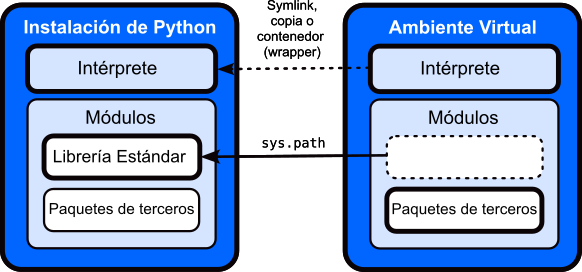
\includegraphics[width=0.5\linewidth]{ambienteVirtual}
\caption{Los ambientes de Python poseen un intérprete y módulos. Los ambientes virtuales comparten el intérprete y la librería estándar con el ambiente global del Python. Tomado y modificado de \citet{jolowicz2024}.}
\label{fig:ambienteVirtual}
\end{figure}
	
%%%%%%%%%%%%%%%%%%%%%%%%%%%%%%%%%%%%%%%%%%%%%%%%%%%
Antes de comenzar la creación de un nuevo ambiente de Python, se recomienda, ampliamente, que se genere una carpeta que almacene subcarpetas, que a su vez, corresponderán a los distintos ambientes que puedan crearse. Para este ejemplo, \texttt{envir\_gar} será la carpeta donde se guardará la subcarpeta con el nuevo ambiente (figura \ref{fig:figura01}).
	
\begin{figure}[H]
\centering
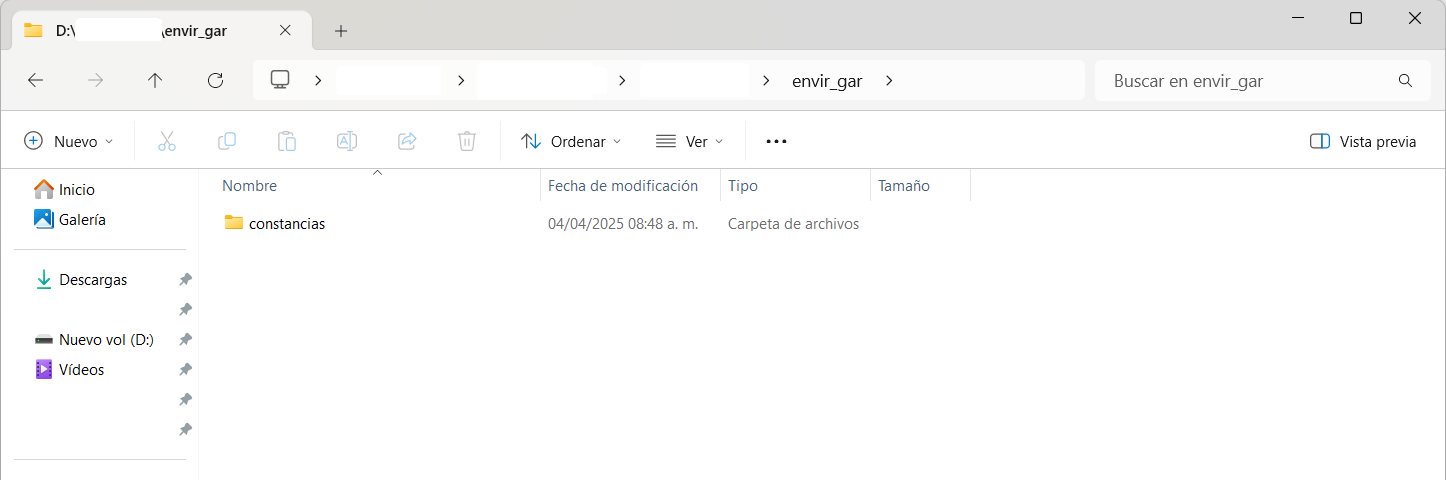
\includegraphics[width=0.8\linewidth]{figura01}
\caption{Carpeta donde se almacenarán las subcarpetas correspondientes a los ambientes virtuales.}
\label{fig:figura01}
\end{figure}
	
Para crear un ambiente, abrimos una ventana de comandos de Python (Windows) y usando el comando \texttt{cd} nos ubicaremos dentro de la carpeta que se mencionó en el párrafo anterior (figuras \ref{fig:figura02} y \ref{fig:figura03}).
\begin{figure}[H]
\centering
\includegraphics[width=0.9\linewidth]{figura02}
\caption{En la ventana de comandos del sistema (Python), usamos el comando cd para  ubicarnos en la carpeta que almacena los ambientes.}
\label{fig:figura02}
\end{figure}
	
\begin{figure}[H]
\centering
\includegraphics[width=0.9\linewidth]{figura03}
\caption{En la ventana de comandos del sistema (Python), nos ubicamos en la carpeta que almacena los ambientes.}
\label{fig:figura03}
\end{figure}
	
Procedemos a crear un ambiente virtual de Python con el nombre de geoanalisis, usando la instrucción antes mencionada (figura \ref{fig:figura04}).
\begin{verbatim}
python -m venv geonalisis
\end{verbatim}
	
\begin{figure}[H]
\centering
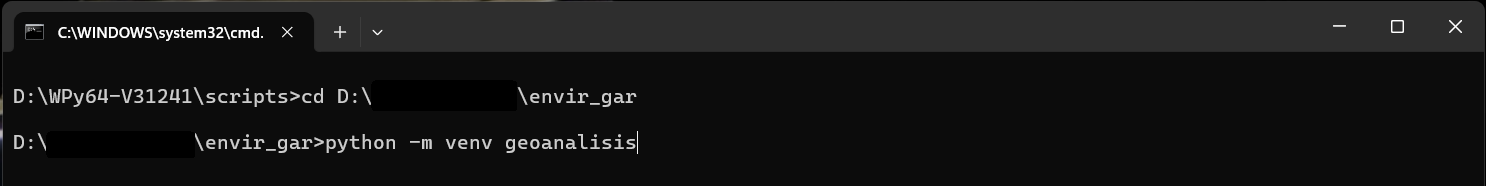
\includegraphics[width=0.9\linewidth]{Figura04}
\caption{Creando el ambiente virtual de Python.}
\label{fig:figura04}
\end{figure}
	
Una vez que proporcionamos la instrucción para crear el ambiente, esperamos un par de segundos y observaremos que el cursor de la ventana de comandos aparecerá de nuevo. Usando el Explorador de Windows podemos identificar que se generó una subcarpeta con el ambiente que ha sido creado unos momentos antes (figura \ref{fig:figura05}).
\begin{figure}[H]
\centering
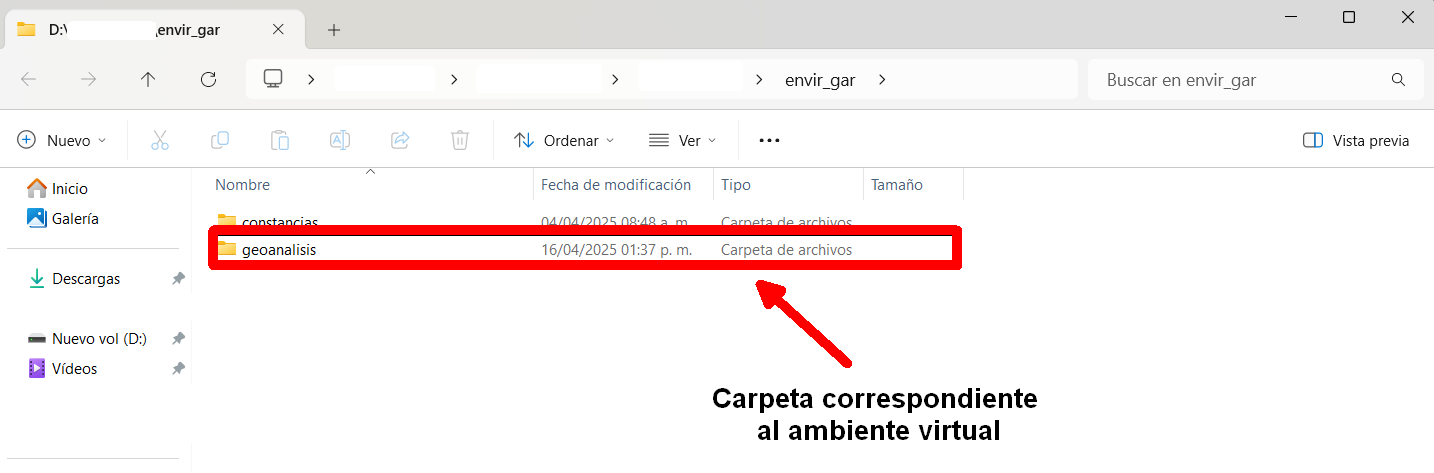
\includegraphics[width=0.9\linewidth]{Figura05}
\caption{El proceso de creación del ambiente virtual generó una subcarpeta con el nombre del ambiente.}
\label{fig:figura05}
\end{figure}
	
Dentro de la subcarpeta del ambiente, se encontrarán 3 subcarpetas (figura \ref{fig:figura06}):
\begin{enumerate}
    \item Subcarpeta \texttt{Include}.
    \item Subcarpeta \texttt{Lib}. 
    \item Subcarpeta \texttt{Scripts}.
\end{enumerate}
	
\begin{figure}[H]
\centering
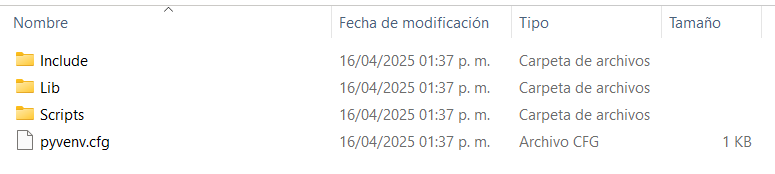
\includegraphics[width=0.8\linewidth]{Figura06}
\caption{Subcarpetas dentro de la carpeta del ambiente virtual, recién creado.}
\label{fig:figura06}
\end{figure}
	
En la subcarpeta \texttt{Include} se guardarán los archivos de las librerías de C, si alguno de los paquetes del ambiente lo requiere; de lo contrario, esta subcarpeta se encontrará vacía.\bigskip
	
Dentro de la subcarpeta \texttt{Lib} encontrarás la subcarpeta \texttt{site-packages}; en esta última carpeta se almacenarán todos los archivos relacionados a los paquetes instalados dentro de este ambiente.\bigskip
	
En la subcarpeta \texttt{Scripts} se ubican 4 archivos que son importantes para usar el ambiente recién creado (figura \ref{fig:figura07}):
\begin{enumerate}\label{listref}
    \item \texttt{activate.bat}. Este archivo de lotes, debe ser invocado para hacer uso del ambiente.
    \item \texttt{deactivate.bat}. Para dejar de usar o abandonar el ambiente este archivo deberá invocarse en la ventana de comandos.
    \item \texttt{pip.exe}. Archivo ejecutable para instalar los paquetes que se emplearán en el ambiente.
    \item \texttt{python.exe}. Archivo ejecutable para invocar el intérprete de Python que se usará dentro del ambiente.
\end{enumerate}
	
\begin{figure}[H]
\centering
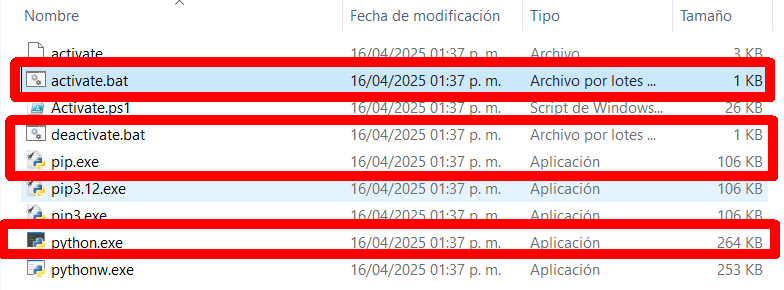
\includegraphics[width=0.8\linewidth]{Figura07}
\caption{Archivos dentro de la carpeta Scripts.}
\label{fig:figura07}
\end{figure}
	
\subsection{Activación del ambiente}
Para comenzar a usar el ambiente es necesario ''activarlo'' y para ello, en la ventana de comandos vamos a ejecutar el archivo \texttt{activate.bat} de la siguiente manera:
\begin{verbatim}
nombre_ambiente\Scripts\activate
\end{verbatim}
	
para nuestro ejemplo, usamos:
\begin{verbatim}
geoanalisis\Scripts\activate
\end{verbatim}
	
Identifica que antes de la ruta de acceso de la ventana de comandos, el sistema agregó el nombre del nuestro ambiente entre paréntesis; indicándonos que ya nos encontramos en el ambiente y podemos realizar nuestro proyecto con los paquetes que se requieran (figura \ref{fig:figura08}).
	
\begin{figure}[H]
\centering
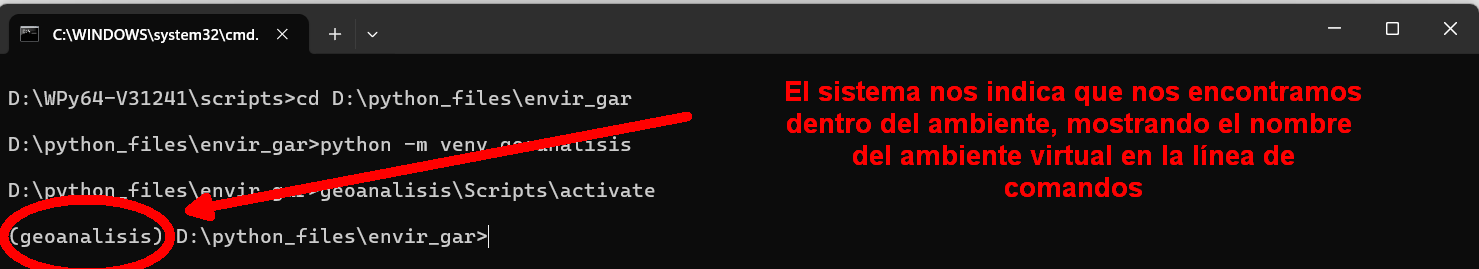
\includegraphics[width=0.9\linewidth]{Figura08}
\caption{Ambiente virtual activado.}
\label{fig:figura08}
\end{figure}
	
\subsection{Instalación de paquetes en el ambiente virtual}
Ya que el ambiente ha sido recién creado, si verificamos los paquetes que se encuentran instalados con el comando \texttt{pip freeze} o \texttt{pip list}, no se visualizará ningún paquete.\bigskip
	
Recordemos que uno de los objetivos en los ambientes virtuales es prevenir conflictos entre versiones de paquetes, por tal razón, inicialmente, el ambiente no cuenta con ninguno y es por ello, debemos instalar los paquetes que requiere nuestro proyecto de Python. La instalación se realiza usando el comando \texttt{pip}. Te recomiendo que consultes las páginas oficiales del paquete para conocer las instrucciones que debes seguir para la instalación de dicho paquete.\bigskip
	
Para este ejemplo, vamos a instalar el paquete de Pandas en nuestro ambiente. Si consultamos la \href{https://pandas.pydata.org/pandas-docs/stable/getting_started/install.html}{página web de instalación de pandas} nos indican que la manera más sencilla de instalar el paquete es por medio de la instrucción (figuras \ref{fig:figura09} y \ref{fig:figura10}):
\begin{verbatim}
pip install pandas
\end{verbatim} 
	
\begin{figure}[H]
\centering
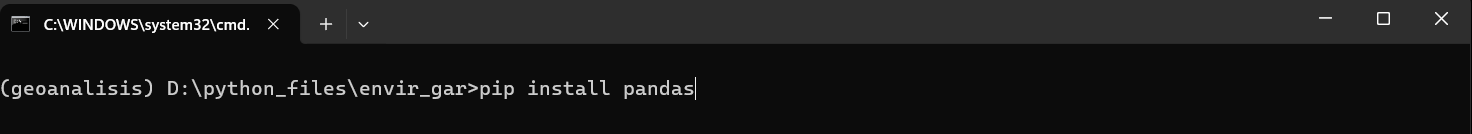
\includegraphics[width=0.9\linewidth]{Figura09}
\caption{Instalando el paquete de Pandas en el ambiente virtual activado.}
\label{fig:figura09}
\end{figure}
	
\begin{figure}[H]
\centering
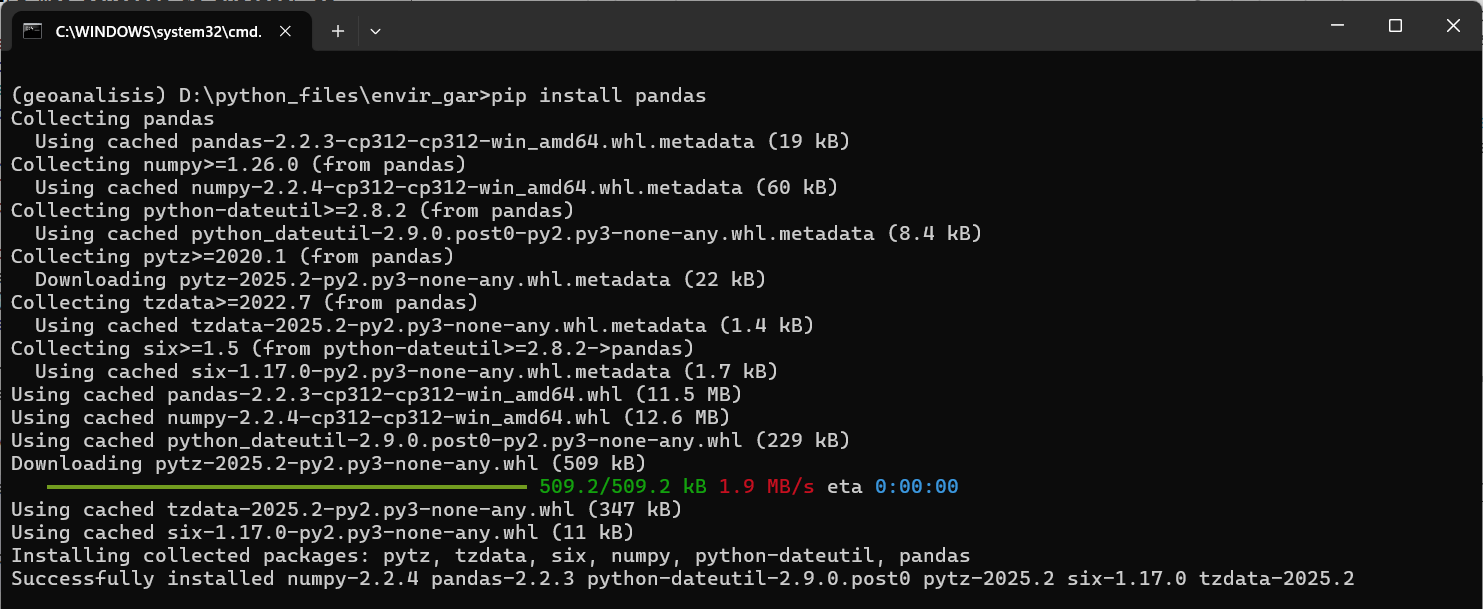
\includegraphics[width=0.9\linewidth]{Figura10}
\caption{Instalación finalizada del paquete.}
\label{fig:figura10}
\end{figure}
	
De hecho en la página web antes mencionada, nos recomiendan que la instalación del paquete se realice en ambientes virtuales.\bigskip
	
Si verificamos de nuevo que paquetes se encuentran instalados en el ambiente, usamos el comando \texttt{pip freeze} y obtendremos un resultado similar al mostrado en la figura \ref{fig:figura11}.
\begin{figure}[H]
\centering
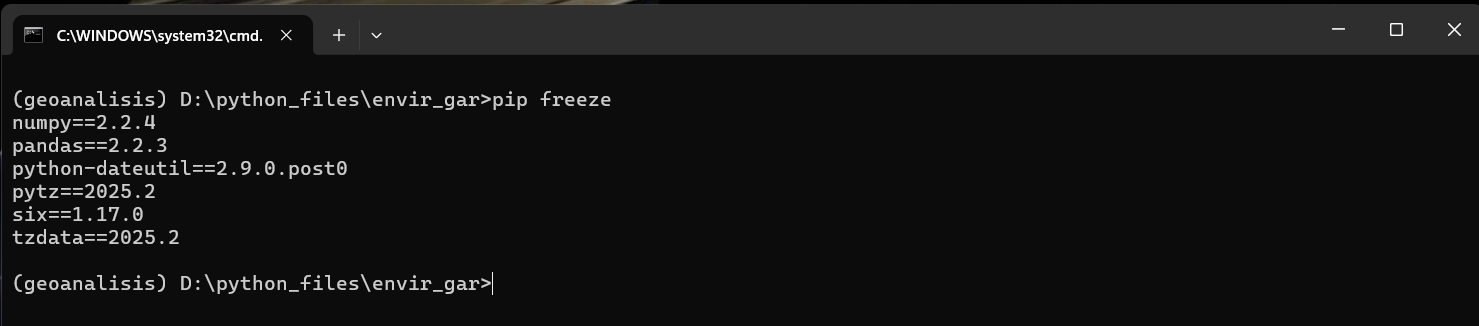
\includegraphics[width=0.9\linewidth]{Figura11}
\caption{Paquetes instalados en el ambiente virtual.}
\label{fig:figura11}
\end{figure}
	
Puede existir el caso donde sea necesario compartir tus programas y estos se encuentran en un ambiente con determinados paquetes. Cuando ocurra esta situación, es recomendable hacer un archivo de requisitos para la instalación de los paquetes. \bigskip
	
En la ventana de comandos del ambiente activo, escribimos las siguiente línea de comandos para generar el archivo de requisitos:
\begin{verbatim}
pip freeze > listapaquetes.txt
\end{verbatim}
	
A las personas que les compartes la lista de los paquetes que tiene tu ambiente, les indicarás que para realizar la instalación con \texttt{pip} deben usar el parámetro \texttt{-f} que precede al nombre del archivo de requisitos, es decir:
\begin{verbatim}
pip install -r listapaquetes.txt
\end{verbatim}
	
%%%%%%%%%%%%%%%%%%%%%%%%%%%%%%%%%%%%%%%%%%%%%%%%%%%
\section{Desactivación del ambiente virtual}
Cuando hemos concluido la programación, desarrollo o ejecución del proyecto relacionado al ambiente, se recomienda que se desactive el ambiente antes de cerrar la ventana de comandos. Para desactivar el ambiente virtual, en la línea de comandos escribimos la siguiente instrucción:
\begin{verbatim}
deactivate
\end{verbatim}
	
Cuando se desactiva el ambiente virtual, el nombre del éste desaparecerá de la línea de comandos (figura \ref{fig:figura12}).
	
\begin{figure}[H]
\centering
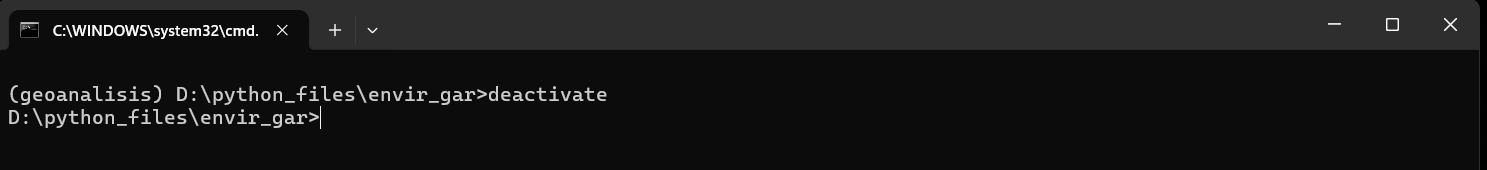
\includegraphics[width=0.9\linewidth]{Figura12}
\caption{Desactivando el ambiente virtual.}
\label{fig:figura12}
\end{figure}
	
%%%%%%%%%%%%%%%%%%%%%%%%%%%%%%%%%%%%%%%%%%%%%%%%%%%
\section{Ambientes virtuales en la distribución de Python Conda (Anaconda)}
Tal como se mencionó anteriormente, se recomienda que tu ubicas dentro de la carpeta donde almacenarás todos tus ambientes y crear subfolder para cada uno de ellos.\bigskip
	
En una ventana de Anaconda Prompt, usamos la siguiente instrucción para crear ambientes virtuales con la distribución de Conda:
\begin{verbatim}
conda create -n nombre_ambiente
\end{verbatim}
	
Y para activar el ambiente, escribimos en la línea de comandos:
\begin{verbatim}
conda activate nombre_ambiente
\end{verbatim}
	
Para desactivar el ambiente, deberás emplear el siguiente comando:
\begin{verbatim}
conda deactivate 
\end{verbatim}
	
Conda permite realizar la creación de un ambiente, así como la instalación de paquetes mediante un archivo \texttt{yaml} (\texttt{*.yml}). En la primera línea se proporciona el nombre del ambiente, en la segunda línea escribimos la palabra ''dependencies'' y en las siguientes líneas se escriben los nombres de los paquetes que se instalarán. Para nuestro ejemplo, la estructura del este archivo es la siguiente:
\begin{verbatim}
name: nombre_ambiente
dependencies:
    - nombre_paquete 
\end{verbatim}
	
Un archivo \texttt{yaml} puede ser creado en cualquier editor de texto, solamente debes de guardar el archivo con la extensión \texttt{.yml}. Para nuestro ejemplo, el archivo tendrá el nombre de geoana.yml y el contenido del archivo \texttt{*.yml} sería:
\begin{verbatim}
name: geoanalisis
dependencies:
    - pandas 
\end{verbatim}
	
Usando este archivo, en Conda Prompt creamos el ambiente con la siguiente instrucción:
\begin{verbatim}
conda env create -f geoana.yml
\end{verbatim}
	
Te recomiendo que consultes las indicaciones que se proporcionan en la pagina web oficial relacionada al tema, que ofrece Conda a los usuarios de esta distribución. La dirección web es:\bigskip
	
\url{https://docs.conda.io/projects/conda/en/stable/user-guide/tasks/manage-environments.html}
	
%%%%%%%%%%%%%%%%%%%%%%%%%%%%%%%%%%%%%%%%%%%%%%%%%%%
\section{Ambientes virtuales en PyCharm}
Debido a la interfase gráfica de usuario que ofrece PyCharm, la creación de ambientes se realiza en el momento que se crea un proyecto nuevo y por tal razón, no es necesario que proporciones de manera manual alguna instrucción o comando para generar un ambiente virtual.\bigskip
	
En la ventana que se abre para generar el proyecto (figura \ref{fig:figura13}), 1) en ''Location'' debes proporcionar la ruta de acceso donde se ubicara la carpeta del proyecto en tu disco duro; 2) en el tipo de intérprete, deberás presionar el botón ''Project venv'' y 3) en ''Python version'' indicas la ruta de acceso del archivo donde se encuentra ejecutable de Python.\bigskip
	
Si PyCharm detecta que en la computadora existe la distribución de Anaconda instalada, entonces en el tipo de intérprete aparece el botón de ''Base Conda''. Si elijes esta opción, en ''Path to Conda'' por default PyCharm coloca la ruta de acceso del intérprete de Python de Anaconda. Identifica que en esta opción no se crea ningún ambiente.\bigskip 
	
Mediante el botón ''Custom environment'' (figura \ref{fig:figura14}), PyCharm te permite la manera de indicar cómo definir el ambiente. Cuando oprimes el botón de personalizar el ambiente, en ''Environment'' aparecen dos opciones: en la primera opción se genera un nuevo (''Generate new'') y en la segunda, se indica el uso de un ambiente, previamente creado ''Select existing''. \bigskip
	
Si creamos un nuevo ambiente, PyCharm nos pide que indiquemos a partir de que tipo (''Type'') vamos a generar el archivo, ya sea con el uso de \texttt{venv} o Conda (figura \ref{fig:figura14}). Si deseamos usar \texttt{venv}, de la lista de tipos seleccionamos ''Virtualenv'' (figura \ref{fig:figura15}). Debemos indicar el intérprete base de Python para nuestro ambiente (ver figura \ref{fig:ambienteVirtual}), así como la ruta de acceso donde se encuentra el archivo ejecutable de Python. En la ubicación del ambiente puedes reconocer que es la misma ruta de acceso del proyecto, solamente que se agrega la carpeta ''venv''. También, la interfase gráfica te ofrece: a) la posibilidad de los paquetes del intérprete base se hereden al nuestro ambiente y b) que el ambiente recién creado se encuentre disponible para todos los proyectos.
	
\begin{figure}[H]
\centering
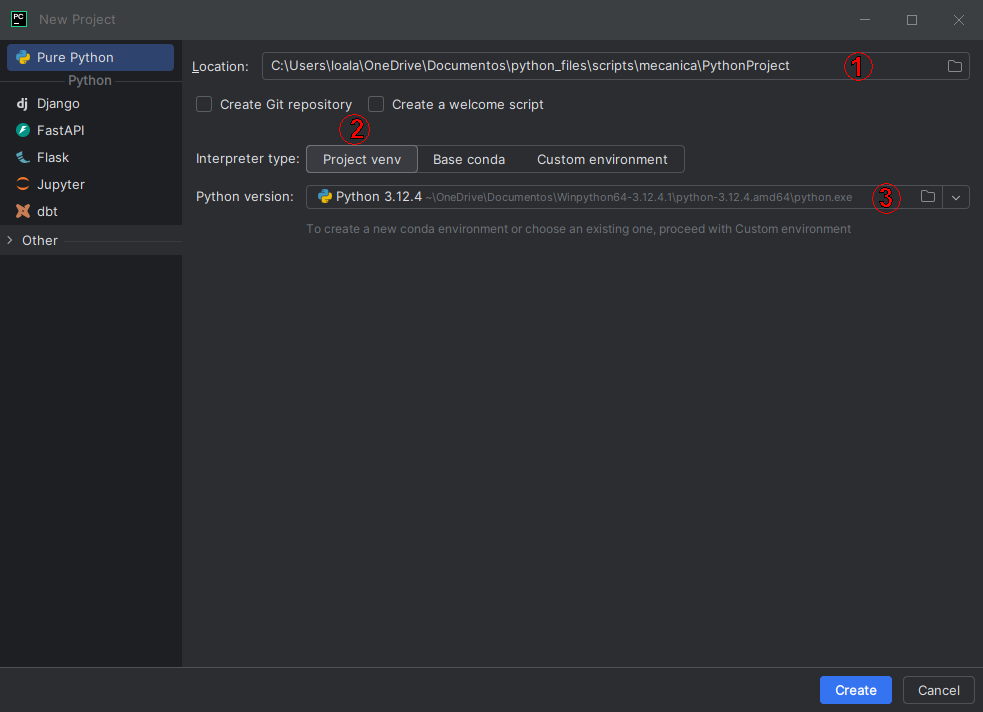
\includegraphics[width=0.8\linewidth]{Figura13}
\caption{Ventana de PyCharm para generar un nuevo proyecto.}
\label{fig:figura13}
\end{figure}
	
\begin{figure}[H]
\centering
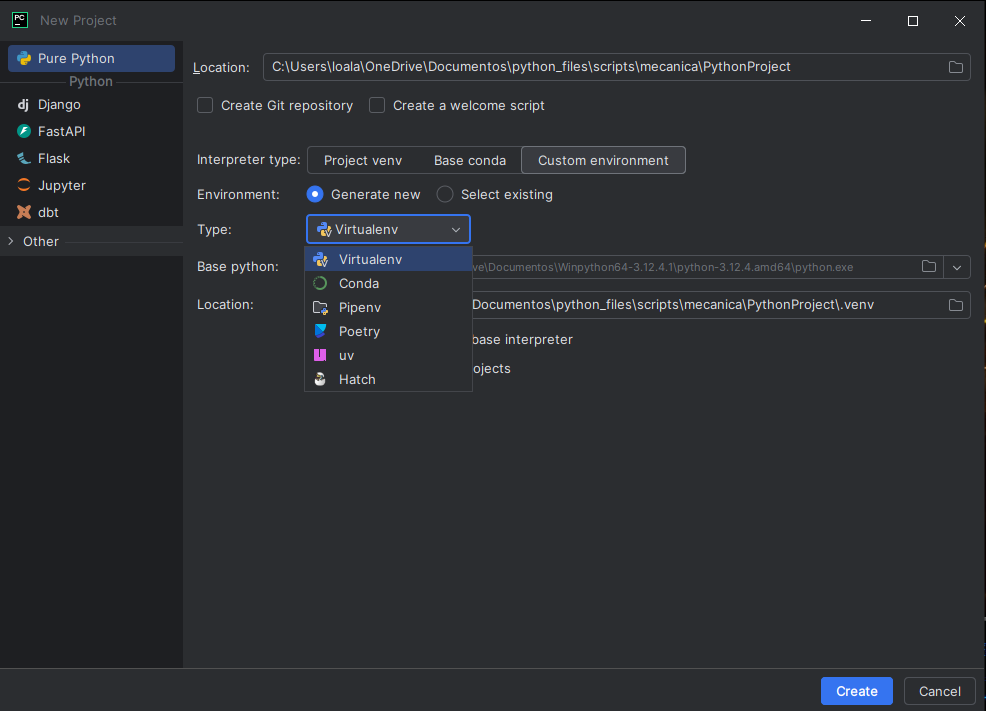
\includegraphics[width=0.8\linewidth]{Figura14}
\caption{Ventana de PyCharm para generar un nuevo proyecto, personalizando la creación del ambiente.}
\label{fig:figura14}
\end{figure}
	
\begin{figure}[H]
\centering
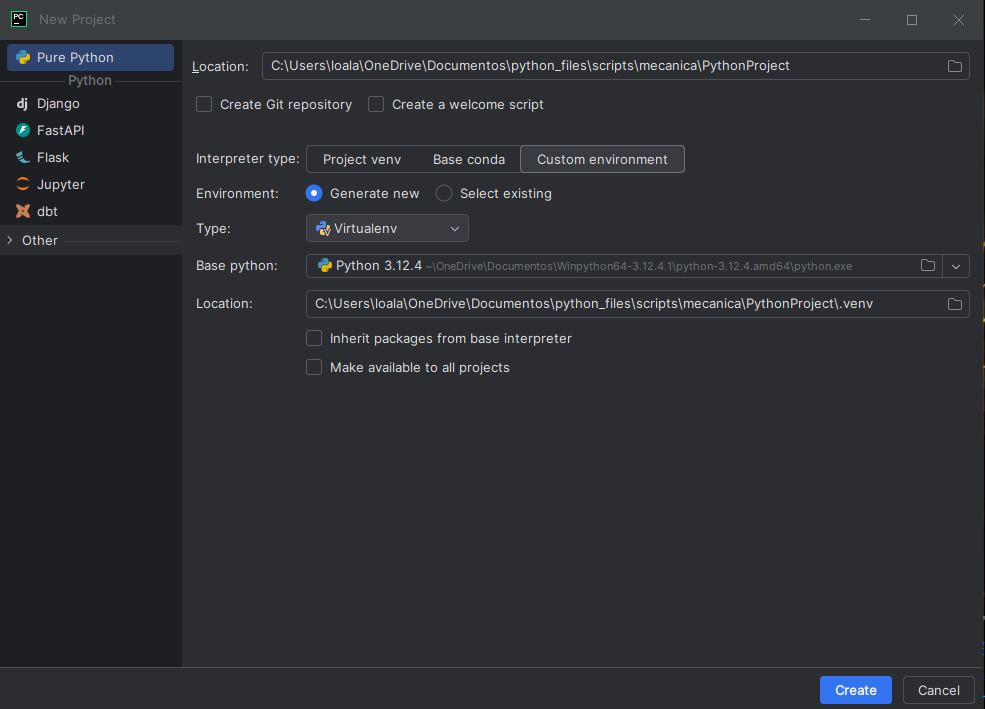
\includegraphics[width=0.8\linewidth]{Figura15}
\caption{Ventana de PyCharm para personalizar el proceso de creación de un ambiente.}
\label{fig:figura15}
\end{figure}
	
Por otra parte, al seleccionar un ambiente existente, debemos indicar la distribución del intérprete de Python, ya sea Python o Conda. Si elegimos Python, debemos indicar la ruta de acceso del archivo ejecutable de Python, el cual se localiza en la subcarpeta \texttt{Scripts} del ambiente (figura \ref{fig:figura06}).
	
%%%%%%%%%%%%%%%%%%%%%%%%%%%%%%%%%%%%%%%%%%%%%%%%%%%
\section{Manejo de ambientes virtuales en Spyder}
En Spyder no es posible crear ambientes virtuales pero mediante el intérprete de Python, que se encuentra en la carpeta de \texttt{Scripts}, puedes hacer uso de los paquetes instalados. \bigskip
	
En la barra de menús de Spyder, selecciona el menu Herramientas y posteriormente, Preferencias; en la ventana que se abre, en el panel izquierdo selecciona y abre Intérprete de Python. Activa la opción de ''Usar el siguiente intérprete'' y proporciona la ruta de acceso del archivo ejecutable de Python de la subcarpeta \texttt{Scripts} del ambiente. Finalizas, oprimiendo el botón de OK (figura \ref{fig:figura16}).\bigskip
	
A continuación, de la barra de menús elige Terminales y de las opciones que se despliegan, deberás elegir ''Reiniciar el núcleo'' (figura \ref{fig:figura17}). \bigskip 
	
Si al efectuar las indicaciones anteriores, en la consola te aparece un mensaje de error mencionando que no es posible usar el núcleo porque no se encuentra el paquete ''spyder-kernels'', cierra Spyder y en la ventana de comandos de Python (Windows), activa el ambiente y procede a instalar el módulo que falta con la  \href{https://pypi.org/project/spyder-kernels/}{siguiente instrucción}:
\begin{verbatim}
pip install spyder-kernels==2.5.*
\end{verbatim}
	
Abre de nuevo Spyder, verifica que el intérprete de Python corresponda al ambiente y para cerciorarte de la disponibilidad de los paquetes, visualiza la lista de módulos con pip freeze.
	
\begin{figure}[H]
\centering
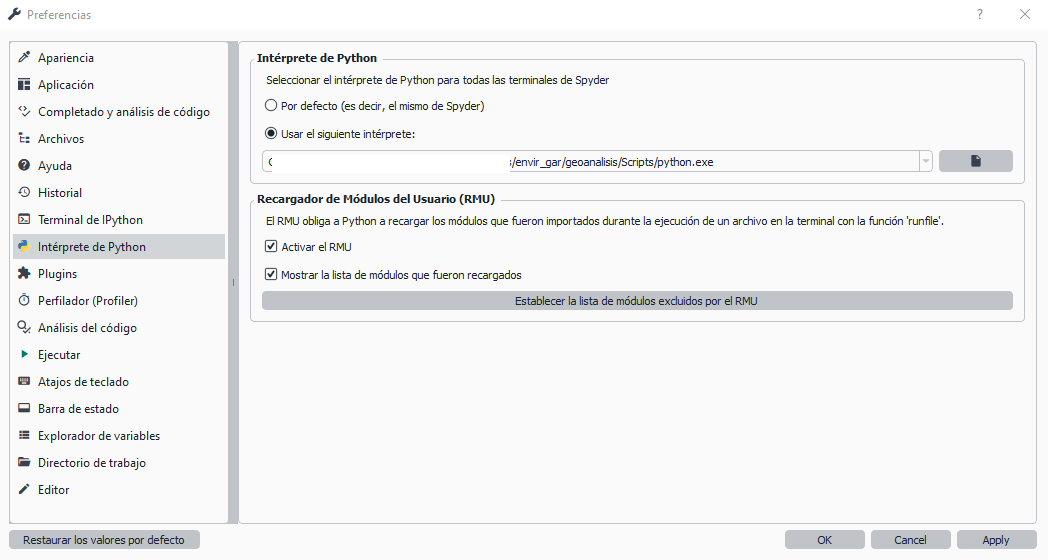
\includegraphics[width=0.8\linewidth]{Figura16}
\caption{Ventana de Spyder para indicar el intérprete de Python.}
\label{fig:figura16}
\end{figure}
	
\begin{figure}[H]
\centering
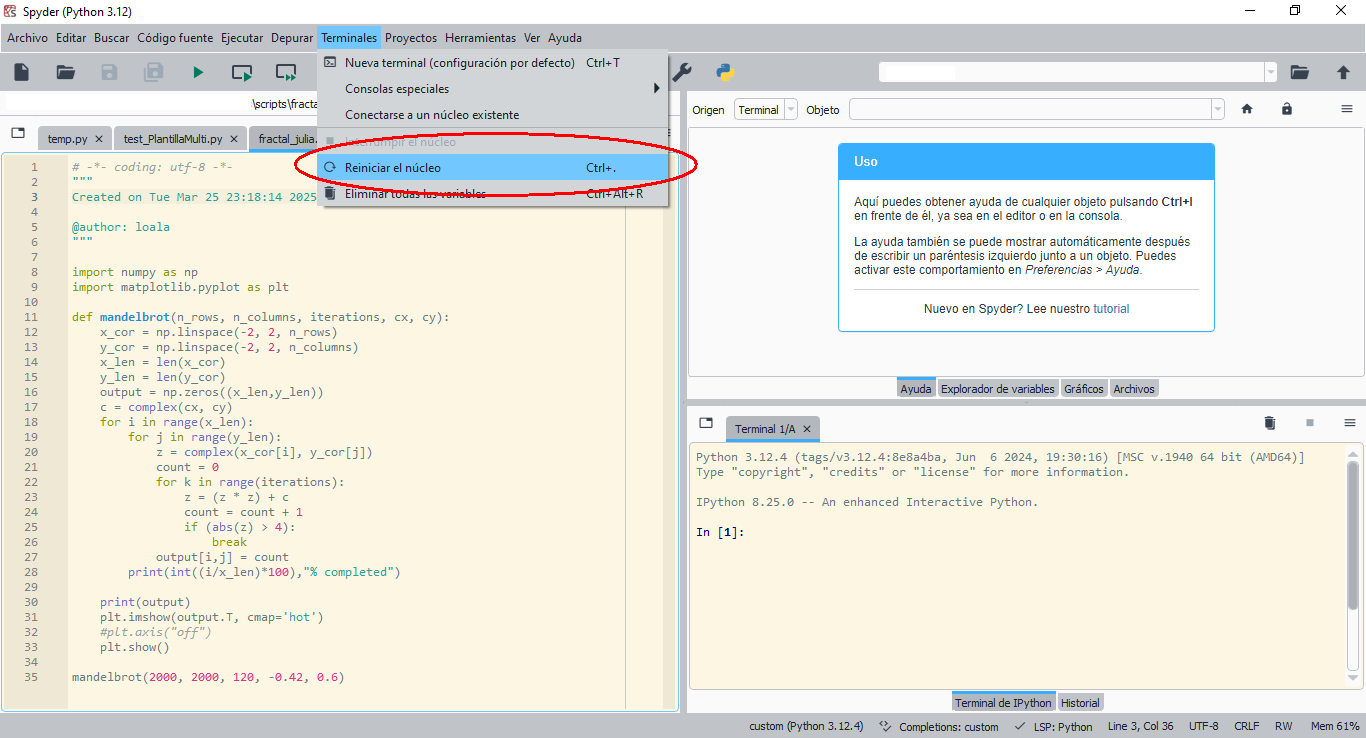
\includegraphics[width=0.9\linewidth]{Figura17}
\caption{Reinicializando el núcleo de la consola de Spyder.}
\label{fig:figura17}
\end{figure}
%%%%%%%%%%%%%%%%%%%%%%%%%%%%%%%%%%%%%%%%%%%%%%%%%%%
\section{Manejo de ambientes virtuales en Visual Studio Code, (VSC)}
De manera similar que en PyCharm, VSC ofrece usar virtualenv de Python y Conda para originar ambientes. Como primer paso vamos a establecer el "workspace" que requiere VSC para crear un ambiente, es por ello que en la barra de menús, elegimos el menu ''File'' y seleccionamos ''Open Folder''; como resultado, la interfase abre una ventana donde ubicaremos la carpeta donde se creará el ambiente. Como ejemplo para este apartado, se creó una carpeta con el nombre de geoanalisisVSC y dicha carpeta fue la elegida como espación de trabajo.\bigskip
	
Una vez elegido la carpeta que almacenará nuestro ambiente, en la barra de menús desplegamos el menu de ''View'' y  en la ''Command Palette'' buscamos y elegimos el comando ''Python: Create Environment'' (figura \ref{fig:figura18}a). A continuación se desplegará una lista donde aparece la opción Venv y Conda (si éste se encuentra instalado en la computadora) (figura \ref{fig:figura18}b). Al seleccionar Venv, visualizamos una lista donde se identifican los intérpretes que podemos usar como base crear el nuevo ambiente (figura \ref{fig:figura19}a). Cuando elegimos intérprete de nuestra elección, VSC comienza a generar de manera autómatica el ambiente, apareciendo en la parte inferior derecha una ventana donde nos notifican que el ambiente está siendo creado (figura \ref{fig:figura19}b).
	
\begin{figure}[H]
\centering
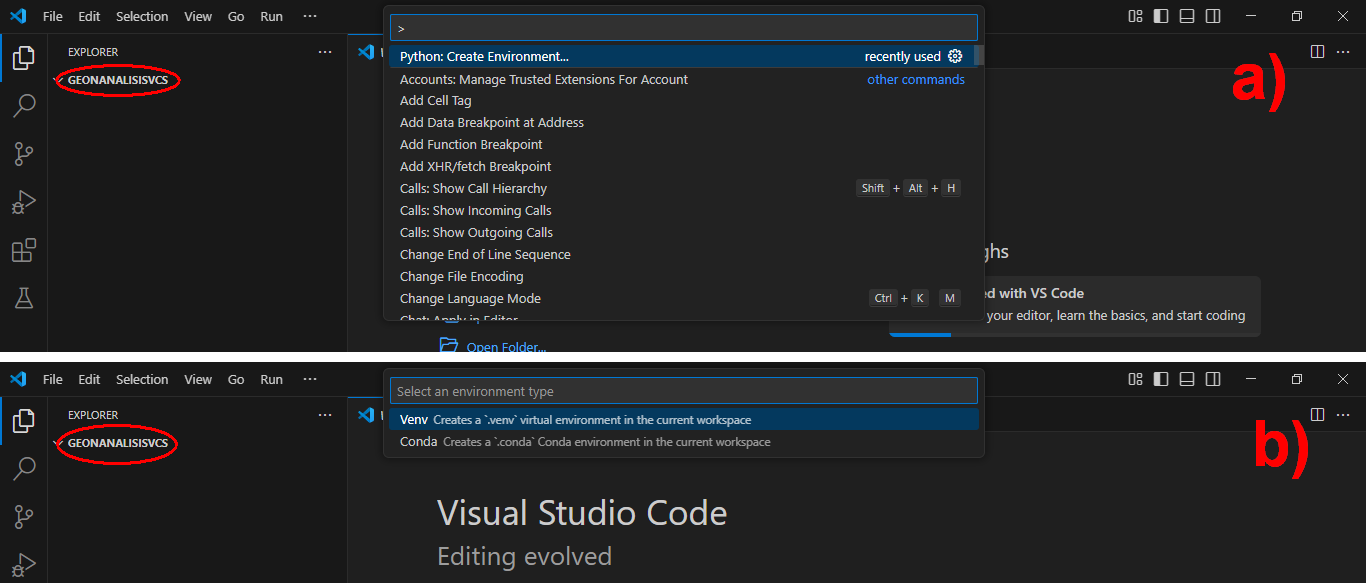
\includegraphics[width=0.9\linewidth]{Figura18}
\caption{a) Paleta de Comandos y búsqueda de comando de creación de ambientes; b) Lista de intérpretes de Python para generar el ambiente.}
\label{fig:figura18}
\end{figure}
	
\begin{figure}[H]
\centering
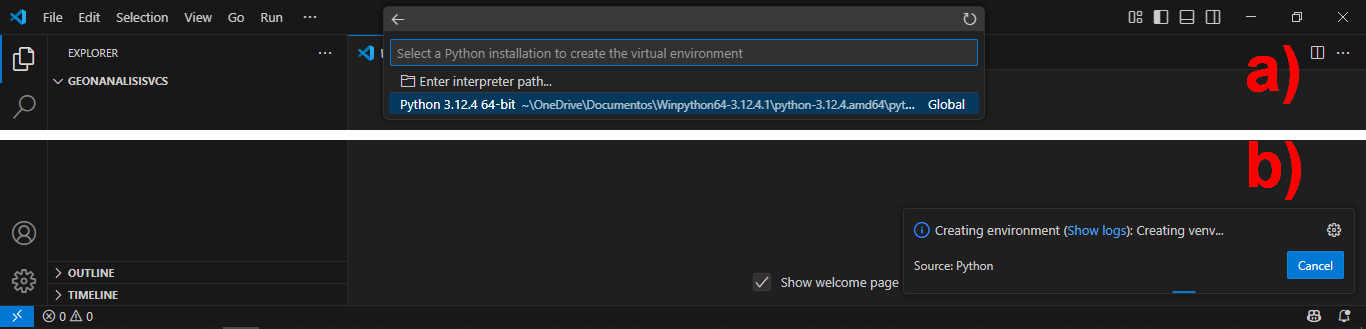
\includegraphics[width=0.9\linewidth]{Figura19}
\caption{a) Paleta de Comandos y búsqueda de comando de creación de ambientes; b) Lista de intérpretes de Python para generar el ambiente.}
\label{fig:figura19}
\end{figure}
	
\begin{figure}[H]
\centering
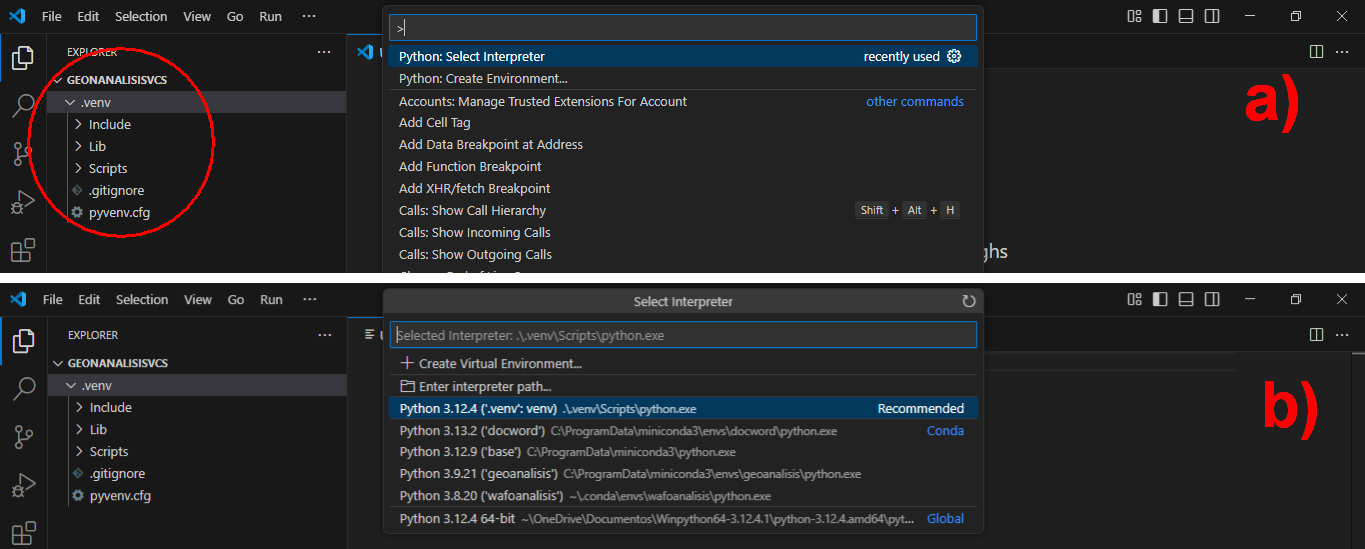
\includegraphics[width=0.9\linewidth]{Figura20}
\caption{a) Seleccionando el intérprete del ambiente,también se resaltan las carpetas recién creadas; b) Eligiendo la opción de búsqueda manual de intérprete de Python.}
\label{fig:figura20}
\end{figure}
	
En la figura \ref{fig:figura20}a se muestra que VSC generó las carpetas Include, Lib, Scripts antes mencionadas. El siguiente paso a seguir será establecer el intérprete del ambiente, que en este caso se ubica en la carpeta de Scripts. De nuevo, abrimos la ''Command Palette'' y buscamos el comando ''Python: select interpreter''; si tenemos más ambientes, una lista con los intérpretes se abrirá, pero en nuestro caso seleccionamos la opción ''Enter interpreter path'' (figura \ref{fig:figura20}b) y se desplegará el comando ''Find... Browse your file system to find a Python interpreter'' lo seleccionamos y se abrirá un ventana del sistema para la carpeta con el archivo ejecutable del intérprete; para nuestro ejemplo, este archivo se encontrará en la carpeta .venv, subcarpeta Scripts, elegimos python.exe y se oprime el botón de ''Select interpreter''. \bigskip  
	
Si abrimos un archivo *.py en VSC, en la parte inferior derecha de la interfase se identifica el intérprete que fue seleccionado en el paso anterior (figura \ref{fig:figura21}).
	
\begin{figure}[H]
\centering
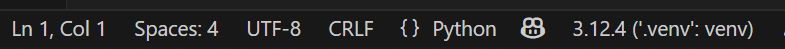
\includegraphics[width=0.7\linewidth]{Figura21}
\caption{En la barra de estado de VCS se identifica el intérprete Python que se encuentra en uso.}
\label{fig:figura21}
\end{figure}
	
%%%%%%%%%%%%%%%%%%%%%%%%%%%%%%%%%%%%%%%%%%%%%%%%%%%
\section{Comentario final}
En esta nota se expone lo que es un ambiente virtual en Python y la manera en la cual se pueden implementar usando diferentes alternativas. Debido a la problemática que se presenta por la dependencia de ciertas versiones de paquetes que requieren los programas, es muy importante para el programador usar los ambientes para eludir conflictos originados por el manejo de diferentes versiones de módulos.\bigskip  
	
Si deseas tener información técnica acerca de cómo funcionan los ambientes virtuales te recomiendo consultes el capítulo 2 del libro de \citet{jolowicz2024}, donde encontrarás con más detalle la administración que realiza Python para el manejo de los ambientes.
	
%%%%%%%%%%%%%%%%%%%%%%%%%%%%%%%%%%%%%%%%%%%%%%%%%%%
\nocite{anaconda2025}
\nocite{python2025}
\nocite{pythont2025}
%\nocite{haber2024}
\nocite{rohowsky2023}
\nocite{vsc2025}
\nocite{mayer2012}
	
% Definiendo el estilo para citar la bibliografia
\bibliographystyle{apalike}
	
% Proporcionando el nombre del archivo bib
\bibliography{referencias}
	
%%%%%%%%%%%%%%%%%%%%%%%%%%%%%%%%%%%%%%%%%%%%%%%%%%%

\vspace{0.5cm}
\hrule 
\vspace{0.25cm}
{\footnotesize Ambientes virtuales en Python © 2025 por Gabriel Ruiz Martínez tiene la licencia CC BY-NC-SA 4.0. Para ver una copia de esta licencia, visita  \url{https://creativecommons.org/licenses/by-nc-sa/4.0/}\bigskip
	
Los ejemplos fueron desarrollados con WinPython 3.12.4.1, MiniConda 25.3.0, Spyder 5.5.5, PyCharm Pro 2025.1, Visual Studio Code 1.99.3. La nota fue creada en \LaTeX{} (TeX Live 2023, TexStudio 4.8.6, compilado con PDFLaTeX) usando la fuente Source Sans Pro; gráficos con Inkscape v.1.4.}